\begin{enumerate}
\item In population ecology there is a partial order ``predates''
which basically means that one organism feeds upon another.  Strictly
speaking this relation is not transitive; however, if we take the point
of view that when a wolf eats a sheep, it is also eating some of the grass
that the sheep has fed upon, we see that in a certain sense it is transitive.
A chain in this partial order is called a ``food chain'' and so-called 
apex predators are said to ``sit atop the food chain''.  Thus ``apex 
predator'' is a term for a maximal element in this poset.   When poisons
such as mercury and PCBs are introduced into an ecosystem, they tend to
collect disproportionately in the apex predators -- which is why pregnant
women and young children should not eat shark or tuna but sardines 
are fine.

Below is a small example of an ecology partially ordered by ``predates''

\begin{center}
\begin{picture}(0,0)%
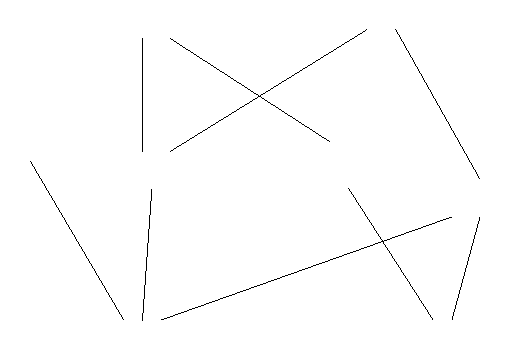
\includegraphics{./ecosystem.pdf}%
\end{picture}%
\setlength{\unitlength}{3947sp}%
%
\begingroup\makeatletter\ifx\SetFigFont\undefined%
\gdef\SetFigFont#1#2#3#4#5{%
  \reset@font\fontsize{#1}{#2pt}%
  \fontfamily{#3}\fontseries{#4}\fontshape{#5}%
  \selectfont}%
\fi\endgroup%
\begin{picture}(4091,2787)(1786,-3376)
\put(2874,-771){\makebox(0,0)[lb]{\smash{{\SetFigFont{12}{14.4}{\rmdefault}{\mddefault}{\updefault}{\color[rgb]{0,0,0}Fox}%
}}}}
\put(4651,-736){\makebox(0,0)[lb]{\smash{{\SetFigFont{12}{14.4}{\rmdefault}{\mddefault}{\updefault}{\color[rgb]{0,0,0}Alligator}%
}}}}
\put(1801,-1786){\makebox(0,0)[lb]{\smash{{\SetFigFont{12}{14.4}{\rmdefault}{\mddefault}{\updefault}{\color[rgb]{0,0,0}Cow}%
}}}}
\put(5401,-2236){\makebox(0,0)[lb]{\smash{{\SetFigFont{12}{14.4}{\rmdefault}{\mddefault}{\updefault}{\color[rgb]{0,0,0}Goose}%
}}}}
\put(2851,-2011){\makebox(0,0)[lb]{\smash{{\SetFigFont{12}{14.4}{\rmdefault}{\mddefault}{\updefault}{\color[rgb]{0,0,0}Duck}%
}}}}
\put(4276,-1936){\makebox(0,0)[lb]{\smash{{\SetFigFont{12}{14.4}{\rmdefault}{\mddefault}{\updefault}{\color[rgb]{0,0,0}Robin}%
}}}}
\put(5101,-3361){\makebox(0,0)[lb]{\smash{{\SetFigFont{12}{14.4}{\rmdefault}{\mddefault}{\updefault}{\color[rgb]{0,0,0}Worms}%
}}}}
\put(2701,-3361){\makebox(0,0)[lb]{\smash{{\SetFigFont{12}{14.4}{\rmdefault}{\mddefault}{\updefault}{\color[rgb]{0,0,0}Grass}%
}}}}
\end{picture}%

\end{center}

Find the largest antichain in this poset.

\newpage

\item Referring to the poset given in exercise 1, match the following.

\begin{tabular}{lr}
\rule{2.3in}{0pt} & \rule{2.3in}{0pt} \\
\begin{minipage}[b]{.4\textwidth}
\begin{enumerate}
\item[1.] An (non-maximal) antichain
\item[2.] A maximal antichain
\item[3.] A maximal element
\item[4.] A (non-maximal) chain
\item[5.] A maximal chain
\item[6.] A cover for ``Worms''
\item[7.] A least element
\item[8.] A minimal element
\end{enumerate}
\end{minipage} 
 & 
\begin{minipage}[b]{.4\textwidth}
\begin{enumerate}
\item[a.] Grass 
\item[b.] Goose
\item[c.] Fox
\item[d.] $\{ \mbox{Grass}, \mbox{Duck} \}$
\item[e.] There isn't one!
\item[f.] $\{ \mbox{Fox}, \mbox{Alligator}, \mbox{Cow} \}$
\item[g.] $\{ \mbox{Cow}, \mbox{Duck}, \mbox{Robin}, \mbox{Goose} \}$
\item[h.] $\{ \mbox{Worms}, \mbox{Robin}, \mbox{Fox} \}$
\end{enumerate} 
\end{minipage} \\
\end{tabular}

\item The graph of the edges of a cube is one in an infinite sequence of 
graphs.  These graphs are defined 
recursively by ``Make two copies of the previous graph then join 
corresponding nodes in the two copies with edges.''  The $0$-dimensional
`cube' is just a single point.  The $1$-dimensional cube is a single edge
with a node at either end.  The $2$-dimensional cube is actually a square
and the $3$-dimensional cube is what we usually mean when we say ``cube.''

\begin{center}
\begin{picture}(0,0)%
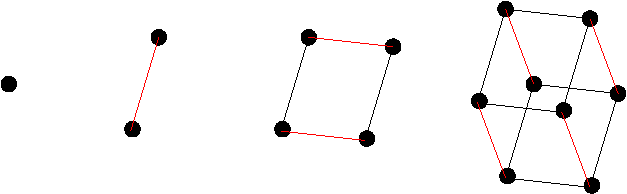
\includegraphics{./0-3_dim_cubes.pdf}%
\end{picture}%
\setlength{\unitlength}{3947sp}%
%
\begingroup\makeatletter\ifx\SetFigFont\undefined%
\gdef\SetFigFont#1#2#3#4#5{%
  \reset@font\fontsize{#1}{#2pt}%
  \fontfamily{#3}\fontseries{#4}\fontshape{#5}%
  \selectfont}%
\fi\endgroup%
\begin{picture}(5015,1548)(1656,-6190)
\end{picture}%

\end{center}

Make a careful drawing of a \index{hypercube}\emph{hypercube} -- which is
the name of the graph that follows the ordinary cube in this sequence.

\item Label the nodes of a hypercube with the divisors of $210$ in order to
produce a Hasse diagram of the poset determined by the divisibility relation.

\item Label the nodes of a hypercube with the subsets of $\{a,b,c,d\}$ 
in order to produce a Hasse diagram of the poset determined by the 
subset containment relation.
  
\item Complete a Hasse diagram for the poset of divisors of 11025 (partially ordered by divisibility).

\item Find a collection of sets so that, when they are partially ordered by $\subseteq$, we obtain the same Hasse diagram as in the previous problem.

\end{enumerate}

%% Emacs customization
%% 
%% Local Variables: ***
%% TeX-master: "GIAM-hw.tex" ***
%% comment-column:0 ***
%% comment-start: "%% "  ***
%% comment-end:"***" ***
%% End: ***
